% ***************** llnlCoverPage.tex ********************************************************************************
% This file defines the following commands for generating the
% front and back cover pages:
%
%     \makeLLNLCover{UCRL}{Title}{Authors}{Journal}{Date}{hShift}{vShift}
%  and
%     \makeLLNLBackCover
%      
% where
%
%  UCRL: The UCRL (6 digit) number (which you probably won't know before the document 
%        is released so just make up a number)
%  Title: title of the article
%  Authors: Authors separated by \\
%  Journal: The journal name
%  Date : the date
%  hShift,vShift : horizontal and vertical shifts to apply to the title page to position it correctly (since
%                  the automatic positioning may not work)
%
% Here is an example:
%  \makeLLNLCover{123456}{An adaptive numerical method for high-speed reactive flows}{William D. Henshaw\\%
%   Donald W. Schwendeman}{Journal of Computational Physics}{January 1, 2003}{0in}{0in}
% 
% *****************************************************************************************************************
% 
\newcommand{\setPageForLLNLCover}[2]{%
\newlength{\textwidthOld}%
\setlength{\textwidthOld}{\textwidth}%
\newlength{\textheightOld}%
\setlength{\textheightOld}{\textheight}%
\newlength{\topmarginOld}%
\setlength{\topmarginOld}{\topmargin}%
\newlength{\textwidthNew}%
\setlength{\textwidthNew}{6.5in}%
\newlength{\textheightNew}%
\setlength{\textheightNew}{9.5in}%
\newlength{\oddsidemarginNew}%
\newlength{\topmarginNew}%
\setlength{\oddsidemarginNew}{(\paperwidth-\textwidthNew)/2 - 1in + #1}%
\setlength{\topmarginNew}{(\paperheight-\textheightNew -\headheight-\headsep-\footskip)/2 - 1in +1.cm + #2}%
\newlength{\oddsidemarginOld}%
\setlength{\oddsidemarginOld}{\oddsidemargin}%
\changepage{\textheightNew-\textheightOld}{\textwidthNew-\textwidthOld}{\oddsidemarginNew-\oddsidemarginOld}{\oddsidemarginNew-\oddsidemarginOld}{}{\topmarginNew-\topmarginOld}{}{}{}%
}%
\newcommand{\setPageForLLNLBackCover}{%
\changepage{\textheightNew-\textheightOld}{\textwidthNew-\textwidthOld}{\oddsidemarginNew-\oddsidemarginOld}{\oddsidemarginNew-\oddsidemarginOld}{}{\topmarginNew-\topmarginOld}{}{}{}%
}%
\newcommand{\resetPageFromLLNLCover}{%
\changepage{-\textheightNew+\textheightOld}{-\textwidthNew+\textwidthOld}{-\oddsidemarginNew+\oddsidemarginOld}{-\oddsidemarginNew+\oddsidemarginOld}{}{-\topmarginNew+\topmarginOld}{}{}{}%
}%
% *************************************************************************************


% *************************************************************************************
\newcommand{\makeLLNLCover}[7]{%
\setPageForLLNLCover{#6}{#7}%
\thispagestyle{empty}% no number of this page
\newcommand{\logoWidth}{1.65in}% 
\psset{xunit=1.cm,yunit=1.cm,runit=1.cm}%
\begin{pspicture}(0,0)(17,24.)
% turn on the grid for placement
% \psgrid[subgriddiv=2]
\rput(2.3,12.5){\epsfig{file=../common/Logo_for_papers.ps,width=\logoWidth}}
\rput(11.2,23.){\parbox{12.0cm}{\large\bf%
\begin{flushright}
% jg - just pass in full UCRL string
%Preprint \\
%UCRL-JC-#1
#1
\end{flushright}
}}
\rput(10.5,18){\parbox{12.0cm}{%\sffamily\bfseries\Huge\noindent%
\fontsize{24.88}{30pt}\usefont{OT1}{cmss}{bx}{n}
\begin{flushleft}
#2
\end{flushleft}
}}
\rput(10.5,13.){\parbox{12.0cm}{%\sffamily\LARGE\noindent%
\fontsize{17.28}{18pt}\usefont{OT1}{cmss}{m}{sl}
\begin{flushleft}
#3
\end{flushleft}
}}
\rput(10.5,9.5){\parbox{12.0cm}{% \sffamily\large\noindent%
\fontsize{14}{16pt}\usefont{OT1}{cmss}{m}{n}
This article was submitted to #4
}}
\rput(10.5,7.5){\parbox{12.0cm}{% \sffamily\bfseries\LARGE\noindent%
\fontsize{20.74}{22pt}\usefont{OT1}{cmss}{bx}{n}
\begin{flushleft}
#5
\end{flushleft}
}}
% \rput[l](4,6.375){\psframebox{\parbox{2.5cm}{\bf%
% \begin{flushleft}
% Lawrence\\
% Livermore\\
% National\\
% Laboratory
% \end{flushleft}
% }}}
\rput(10.5,-1.){\parbox{12.0cm}{%
Approved for public release; further dissemination unlimited}}
\end{pspicture}
% }
%
\clearpage 
% -------------- back of front cover -------------------------
\changetext{.625in}{}{}{}{}
\thispagestyle{empty}% no number of this page
\vglue5\baselineskip
\begin{center}
{\bf DISCLAIMER}
\end{center}
\noindent
% jg - updated disclaimer for report format
This document was prepared as an account of work sponsored by an
agency of the United States Government.  Neither the United States
Government nor the University of California nor any of their
employees, makes any warranty, express or implied, or assumes any
legal liability or responsibility for the accuracy, completeness, or
usefulness of any information, apparatus, product, or process
disclosed, or represents that its use would not infringe privately
owned rights. Reference herein to any specific commercial product,
process, or service by trade name, trademark, manufacturer, or
otherwise, does not necessarily constitute or imply its endorsement,
recommendation, or favoring by the United States Government or the
University of California.  The views and opinions of authors expressed
herein do not necessarily state or reflect those of the United States
Government or the University of California, and shall not be used for
advertising or product endorsement purposes.
\vskip2\baselineskip
\noindent
This work was performed under the auspices of the U. S. Department of
Energy by the University of California, Lawrence Livermore National
Laboratory under Contract No. W-7405-Eng-48.
\vskip1\baselineskip
\vfill
\clearpage
\changetext{-.625in}{}{}{}{}
\resetPageFromLLNLCover
\setcounter{page}{1}
% -----------------------------------------------------------------------------------
}
% *************************************************************************************


% *************************************************************************************
\newcommand{\makeLLNLBackCover}{%
\clearpage
\setPageForLLNLBackCover
% jg - suppress printing of essentially blank page here 
%\changetext{.625in}{}{}{}{}
%\thispagestyle{empty}% no number of this page
\ \ 
%\vfill
%\begin{center}
%Approved for public release; further dissemination unlimited
%\end{center}
%\clearpage 
%\clearpage
%\changetext{-.625in}{}{}{}{}
% ---------------------------------------------------------------------------
\thispagestyle{empty}% no number of this page
\renewcommand{\logoWidth}{10.in}
% \vglue\vShift
% \hglue\hShift
\begin{pspicture}(0,0)(17,24.)
% turn on the grid for placement
% \psgrid[subgriddiv=2]
\rput{90}(2.3,12.5){\epsfig{file=../common/Rule_and_address.ps,width=\logoWidth}}
% \rput*[l]{90}(5.5,0){\psframebox{\parbox{8.0cm}{\large%
% \begin{flushleft}
% University of California\\
% Lawrence Livermore National Laboratory\\
% Technical Information Department\\
% Livermore, CA 94551
% \end{flushleft}
% }}}
\end{pspicture}
% \setlength{\textwidth}{4.in}      % page width
% \setlength{\textheight}{8.in}    % page height
\clearpage
\resetPageFromLLNLCover
% -----------------------------------------------------------------------------------
}
% *************************************************************************************




